% Chapter 4
\chapter{نتیجه‌گیری و پیشنهادها}


در این فصل، به ارزیابی مدل در برابر معیارهای مختلف پرداخته می‌شود و دقت‌ به دست آمده توسط مدل روی داده‌های تست گزارش می‌شود. لازم به ذکر است همان‌طور که گفته شد، در هر دور از یادگیری فدرال، ۵۰۰۰۰ تصویر برای آموزش و ۱۰۰۰۰ تصویر برای ارزیابی در نظر گرفته شده است.

\section{معرفی معیارهای مختلف}

شاخص‌های ارزیابی به شرح زیر است:

\begin{itemize}
    \item \textbf{\lr{TP}\LTRfootnote{True Positive}}: موارد مثبت که به درستی طبقه‌بندی شده‌اند.
    \item \textbf{\lr{TN}\LTRfootnote{True Negative}}: موارد منفی که به درستی طبقه‌بندی شده‌اند.
    \item \textbf{\lr{FN}\LTRfootnote{False Negative}}: موارد مثبت که به طور نادرست طبقه‌بندی شده‌اند.
    \item \textbf{\lr{FP}\LTRfootnote{False Positive}}: موارد منفی که به طور نادرست طبقه‌بندی شده‌اند.
\end{itemize}

البته باید توجه داشت که این تعاریف برای مسائل با دو دسته تعریف می‌شوند، اما برای مسائل چند دسته (مانند مسئله جاری) هم قابل تعمیم است. در \cite{b9} به دو مورد از این روش‌ها پرداخته شده است. در این گونه مسائل فقط ابعاد ماتریس درهم‌ریختگی\LTRfootnote{Confusion Matrix} اضافه می‌شود و کلیت مدل تغییر نمی‌کند.

\begin{figure}[H]
    \centering
   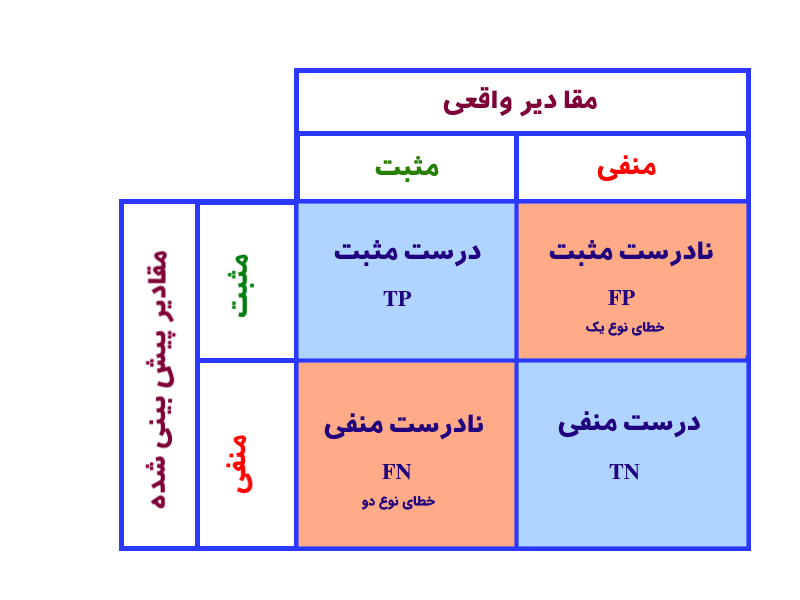
\includegraphics[height=8cm,width=10cm]{./confusion/Actual_Predicted.png}
   \caption{ ماتریس درهم‌ریختگی برای مسئله با دو دسته}
   \label{Confusion}
   \centering
\end{figure}

دقت: این معیار بیانگر دقت کل طبقه‌بندی است و بیانگر نرخ طبقه‌بندی صحیح است. همان‌طور که در رابطه \ref{eq:accuracy} مشاهده می‌شود. تمامی مفاهیم فوق در این رابطه اثر گذارند.

\begin{equation}
    \label{eq:accuracy}
    \text{Accuracy} = \frac{TP+TN}{TP+TN+FP+FN}
\end{equation}




خطا: از این معیار در کنار معیارهای دیگر استفاده می‌شود و بیانگر مقدار فاصله از مقادیر واقعی هر نمونه برای پیش‌بینی توسط مدل است. در رابطه \ref{eq:loss} نماد M بیانگر تعداد کلاس‌ها است و log لگاریتم طبیعی است.  $y_{o,c}$ یک نشانگر دودویی (0 یا 1) است اگر برچسب کلاس c طبقه‌بندی صحیح برای مشاهده o باشد ( برچسب‌های از قبل دانسته) و $p_{o,c}$ احتمال پیش‌بینی شده‌ای است که مشاهده o از کلاس c باشد (برچسب های پیش‌بینی).

\begin{equation} 
\label{eq:loss} 
\text{Loss}=-\sum_{c=1}^My_{o,c}\log(p_{o,c}) 
\end{equation}

\section{نتایج به‌دست آمده}

در ادامه به تاثیر دو پارامتر تعداد کارگران و تعداد دور‌های آموزشی بر هر یک از معیار‌های دقت و خطای کل مدل شبکه عصبی فرآیند یادگیری فدرال پرداخته شده است. به عنوان نمونه در این شبیه‌سازی یک‌ بار با ۱۰ کارگر و بار دیگر با ۵ کارگر اجرا شده است. لازم به ذکر است که نتایج آورده شده حالت محدودی از یک سناریو واقعی اینترنت اشیاء است که میتواند گاهاً تا هزاران دستگاه کم توان روی شبکه را نیز در بر بگیرد. در این آزمایش به دلیل کمبود منابع سخت افزاری و زمانی این تعداد را به اندازه یک شبکه داخلی (مثلا خانه هوشمند) محدود شده‌ است. طبق \cite{b12} میانگین تعداد این دستگاه‌ها در کشور ژاپن در هر خانه برابر با ۱۰.۳ عدد است که باتوجه کمتر بودن این عدد در کشور ایران، یکبار با ۷ عدد و بار دیگر با ۱۰ عدد شبیه ‌سازی شده است. در ادامه نمودار‌های مرتبط با نتایج این شبیه‌سازی در تصاویر \ref{ acc } و \ref{ loss } برای شهود بیشتر و بهتر آورده شده است.

\begin{figure}[H]
    \centering
   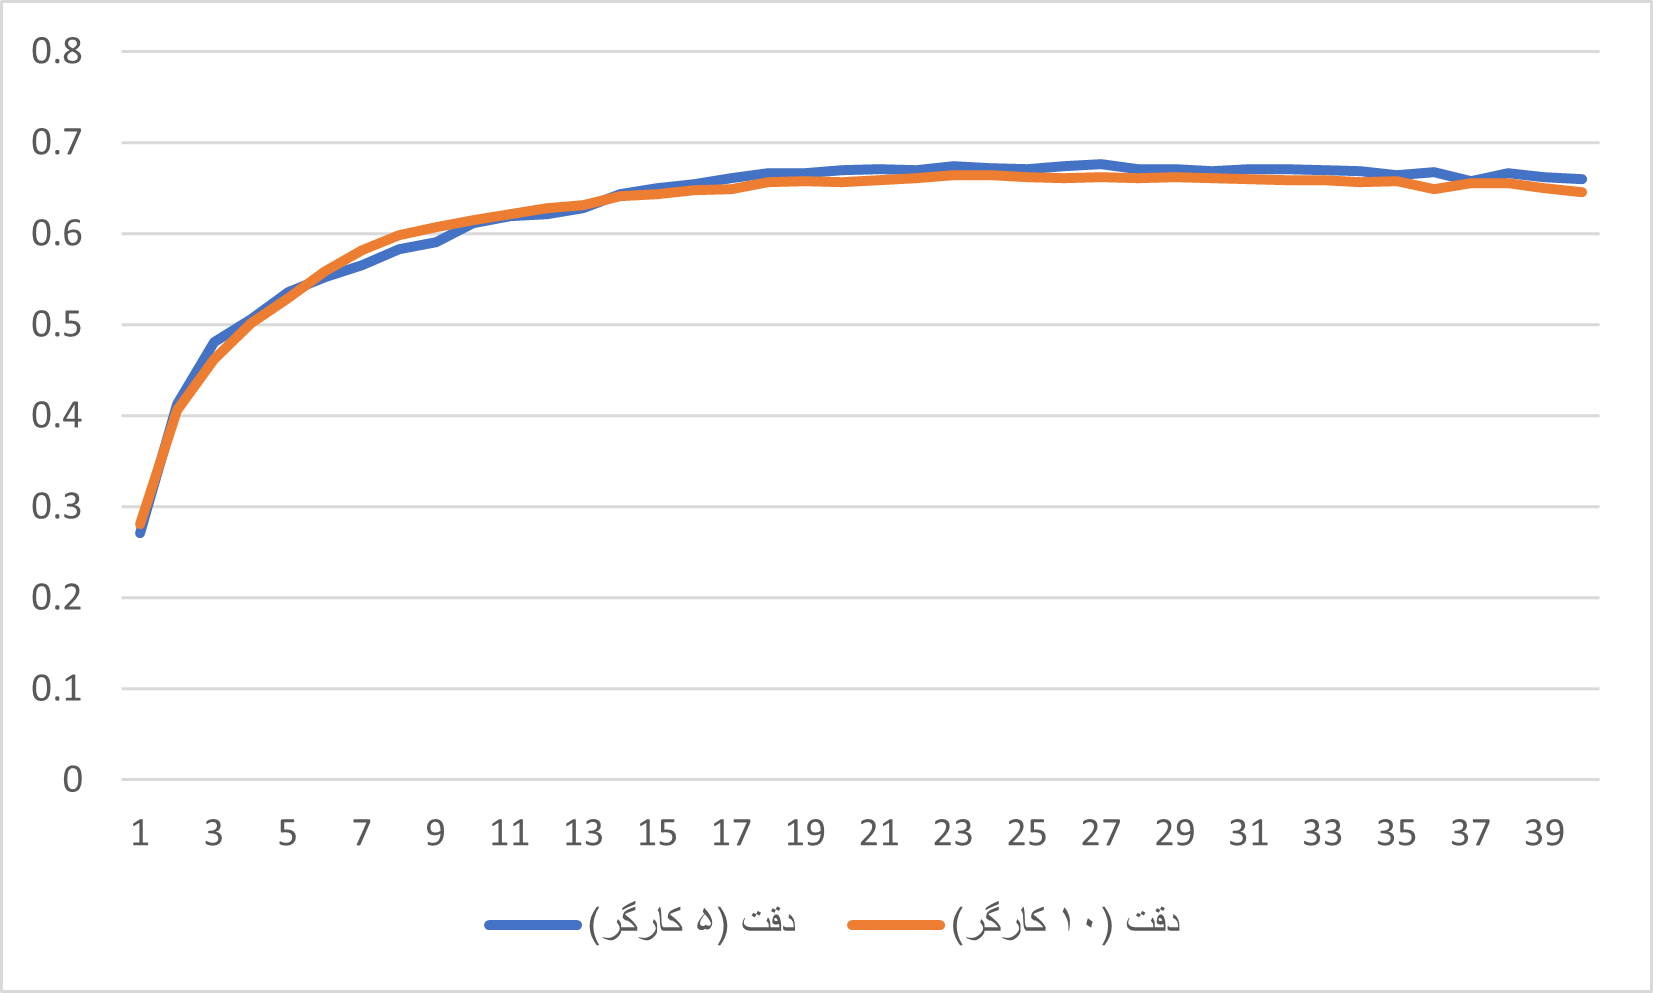
\includegraphics[height=10cm,width=14cm]{./charts/acc.png}
   \caption{ نمودار دقت به‌دست آمده در هر دور از آموزش سراسری}
   \label{ acc }
   \centering
\end{figure}

\begin{figure}[H]
    \centering
   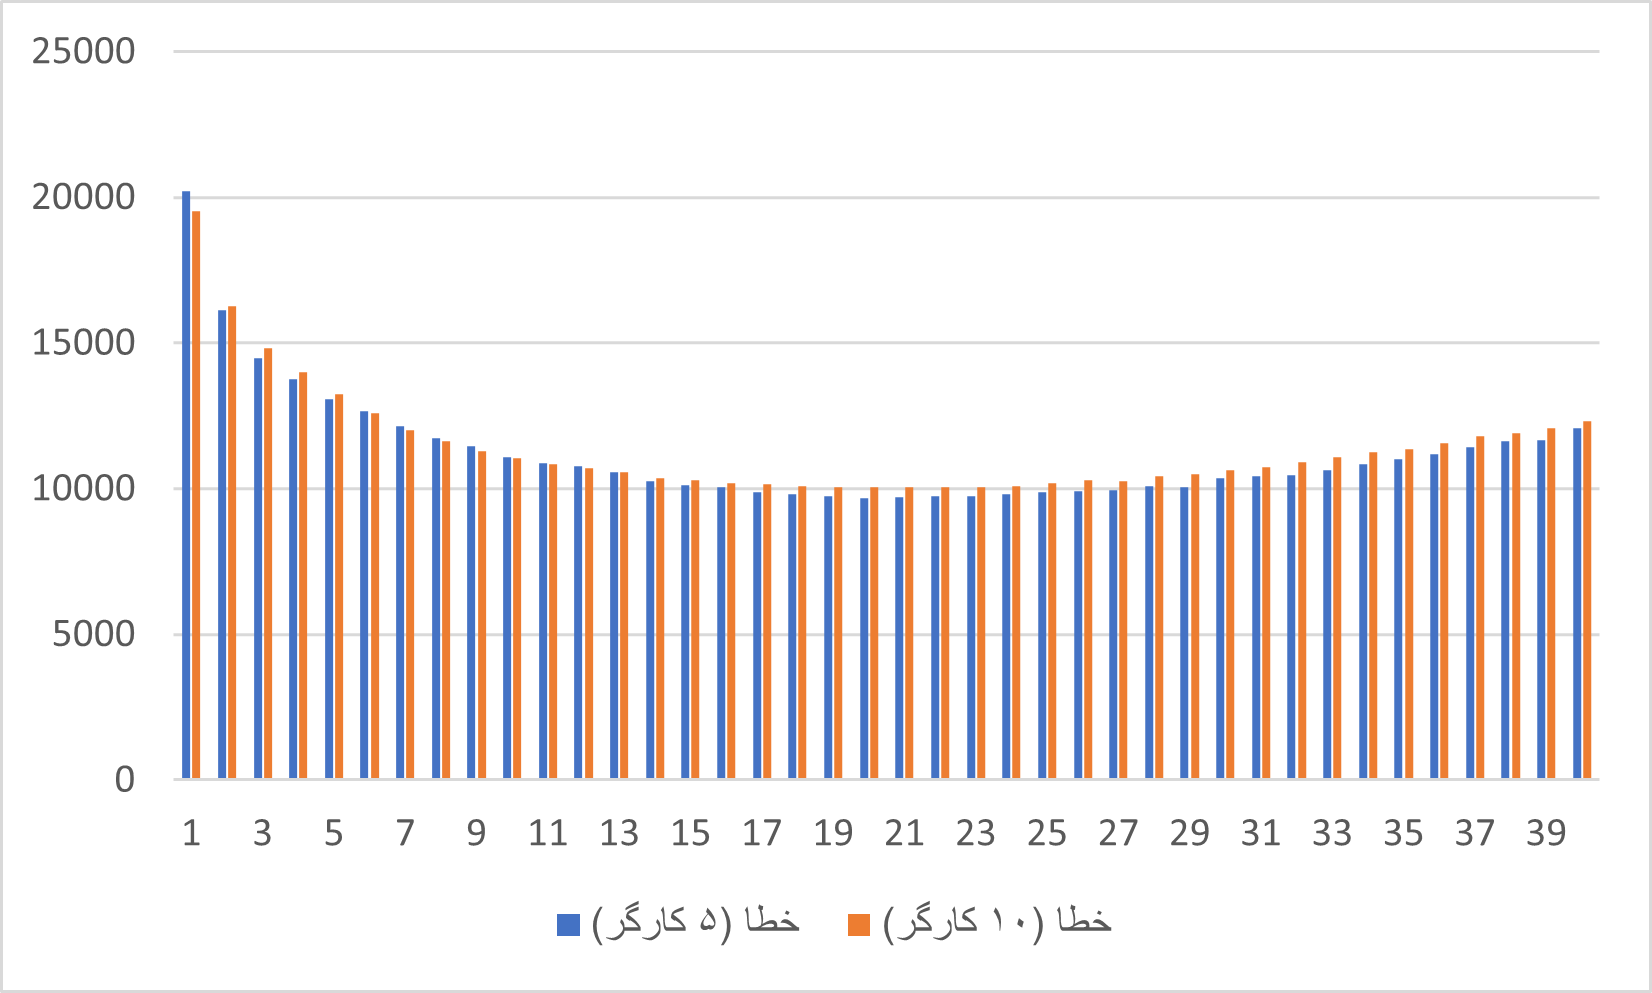
\includegraphics[height=10cm,width=14cm]{./charts/loss.png}
   \caption{ نمودار خطا در هر دور از آموزش سراسری }
   \label{ loss }
   \centering
\end{figure}

همان‌طور که از نمودار‌ها مشخص است، فرآیند آموزش در ابتدا سرعت بالایی دارد و در ادامه به یک خط مماس با شیب نسبتاً کم همگرا می‌شود تا در نهایت به صفر میل کند. با توجه به اینکه این فرآیند دو بار و با تعداد کارگران مختلف انجام شده است، می‌توان دید که تعداد دور آموزشی رابطه مستقیم بیشتری با تعداد کارگران دارد. البته اگر از یک استراتژی داینامیک به جای FedAVG استفاده شود، توقع داریم که به دقت‌های بالاتری برسیم و حتی سرعت همگرایی نیز با شیب بیشتری طی شود.

نمودار دوم گویای این است که طی یک روند غیرخطی در دور ۱۹ام به نقطه کمینه از نظر خطای مدل دسته‌بندی کننده می‌رسیم و در ادامه این روند رو به افزایش است. این می‌تواند بیانگر این باشد که آموزش بیشتر باعث می‌شود شبکه عصبی استفاده شده به عنوان مدل، رو به بیش برازش\LTRfootnote{Overfitting} شدن برود. همان‌طور که می‌دانیم ذات شبکه عصبی با آموزش زیاد به شدت مستعد بیش‌برازش شدن است. در \cite{bookG} روش‌هایی آورده شده تا با این‌ گونه رفتار مقابله شود.

نکته حائز اهمیت در این شبیه‌سازی این است که زمان تقریبی این شبیه‌سازی با ۱۰ کارگر در ۴۰ دور حدوداً ۴۵ دقیقه می‌باشد که زمان نسبتاً کمی در مقایسه با ماهیت یادگیری فدرال دارد. طبیعتاً در پیاده‌سازی‌های واقعی در شبکه‌های اینترنت اشیاء این زمان نمایی افزایش پیدا می‌کند.

\section{ پیشنهادها برای آینده}

همان‌طور که مشاهده شد، با قرار دادن یک لایه اضافه‌تر انتزاع\LTRfootnote{Abstraction} تحت عنوان لایه پردازش لبه در شبکه‌های اینترنت اشیاء‌ای که از یادگیری فدرال برای پیش‌بردن اهداف مدیرتی و تصمیم‌گیری خود استفاده می‌کنند، می‌توان کنترل و انعطاف‌پذیری بیشتری به شبکه داد. همان‌طور که دیده‌ شد، اضافه شدن این لایه به دلیل اینکه در دقت و کیفیت مدل استفاده شده داخل فرآیند یادگیری نسبت به عدم وجود آن حداقل پس‌رفتی به وجود نمی‌آورد و امید داریم که بهتر از قبل هم باشد، یک کار ارزشمند است. همچنین با اضافه شدن سرور لبه به سیستم یادگیری فدرال، دست برنامه‌نویسان نرم‌افزار نیز برای توسعه برنامه‌های کاربردی روی این شبکه‌ها به مراتب بازتر است.


اگرچه چندین راه حل تحقیقاتی برای کاهش چالش‌های اجرای یک سناریو خاص یادگیری فدرال  در شبکه شامل دستگاه‌های پردازش لبه پیشنهاد شده است، اما هنوز چالش‌هایی وجود دارد که حل نشده‌اند. علاوه بر ابتکارات تحقیقاتی گزارش شده در قسمت‌‌های قبلی، ایده‌های نوین قابل بحثی وجود دارند که در زیر توضیح داده شده است:
 
• فرآیند آموزش یادگیری فدرال با پشتیبانی چند مدل: در فرآیند آموزش یادگیری فدرال، فرض می‌شود که کارگران شرکت‌کننده پارامترهای مدل متناظر خود را با توجه به یک مدل سراسری به‌روز می‌کنند. با این حال، ممکن است کارگران بخواهند چندین مدل را حتی در زمان بطالت خود آموزش دهند؛ بنابراین، جداسازی جمع‌آوری مدل سراسری از آموزش محلی به کارگران اجازه می‌دهد تا از الگوریتم‌های یادگیری مختلف استفاده کنند. به عنوان مثال، ممکن است لازم باشد هم‌زمان چندین مدل مختلف با استفاده از روش فدرال برای اهداف مختلف توسعه یابند؛ بنابراین، تکنولوژی‌های مناسب بایستى تجزیه و تحلیل و پیاده‌سازی شود.
 
• تأثیر کانال شبکه بى‌سیم: دستگاه‌های لبه اغلب از طریق کانال‌های بی‌سیم به سرویس‌دهنده‌های لبه یا ابرى وصل شده‌اند؛ بنابراین، بررسى تأثیر الزامات شبکه، به ویژۀ ارتباطات بی‌سیم، در دقت آموزش مدل فدرال به‌عنوان یک روند تحقیقاتى آینده در نظر گرفتۀ شده است. نویز، خسارت مسیر، ترافیک بالا و قطعی همۀ نقص‌هایی هستند که بایستى در سیستم‌های ارتباطات بی‌سیم در نظر گرفتۀ شود. باید توجه داشت که در سناریو‌های اینترنت اشیاء نیز قطع و وصل شدن دستگاه‌های انتهایی خود دلیلی محکم بر این تأثیرات مخرب می‌باشد.

• انتخاب پویای کارگران و جمع‌آوری تطبیقى مدل: جمع‌آوری مدل تطبیقى و انتخاب مشترى پویا برای تخصیص منابع با در نظر گرفتن رفتار ناهمگون داده، قدرت محاسباتى، اندازۀ داده، ظرفیت شبکه و قابلیت اطمینان لینک در بین کارهای تحقیقاتى آینده قرار دارد. بنابراین، بایستى به‌ عنوان روندهای تحقیقاتی آینده، انتخاب پویای کارگران و جمع‌آوری تطبیقى مدل را بررسى کرد. به ‌عنوان ‌مثال، الگوریتم‌ها و پیچیدگی‌های مناسب برای درخواست‌های پویا کارگر و منابع ناهمگون در هر دو سمت کارگر و سرور اصلی دهنده. در چنین سناریوهایی، باید بتوان فرآیند آموزش یادگیری فدرال را مدیریت کرد. یکی از ایده‌های تعیین ضرایب و پارامتر‌ها برای انتخاب پویا کارگران و جمع‌آوری تطبیقى مدل، تخمین‌زدن تقریبی و تنظیم آن در سرور لبه می‌باشد. این محل که در مرکز شبکه اینترنت اشیاء قرار دارد، تخمین خوبی از رفتار کلی شبکه در اختیار الگوریتم‌های تنظیم‌کننده پارامتر‌ها قرار می‌دهد\cite{a13}.

• روش جدید یادگیری فدرال: اندازه مدل یادگیری فدرال بسیار بزرگ است تا بتواند در یک دستگاه لبه با منابع محدود جا شود. علاوه بر این، آموزش مدل یادگیری فدرال بسیار کند است و نمی‌تواند به همگرایى برسد و نیازهای تأخیر در برخى از برنامه‌های حساس به تأخیر را برآورده کند. روش جدید یادگیری فدرال موردنیاز است تا به طور پویا اهداف را دستیابی کند؛ بنابراین، یادگیرى فدرال پویا و تطبیقى بایستى برای دستگاه‌های لبه با منابع محدود تجزیه و تحلیل و پیاده سازى شود. به عنوان مثال میتوان با وزن دادن به گره‌ها در الگوریتم FedAVG و میانگین وزن‌دار گرفتن از آن‌ها در حین اجرای سیستم، به دقت و سرعت بالاتری دست پیدا کرد.

• پیاده‌سازی پروتکل‌های پیچیده به‌منظور بهبود کیفیت ارتباطات در فرآیند یادگیری: می‌توان از پروتکل‌های مختلف که بعضی سنگین و بعضی دیگر سبک هستند به‌منظور ایجاد یک پروسه یادگیری امن و مطلوب در بستر شبکه استفاده کرد. پیاده‌سازی این پروتکل‌ها می‌تواند معطوف به دستگاه‌های انتهایی نباشد و سرور لبه نیز در آن نقش مشخصی داشته باشد. یکی از این پروتکل‌ها که بدون در نظر گرفتن سرور لبه توسعه پیدا کرده پروتکل SAFA\LTRfootnote{Semi-Asynchronous Protocol for Fast Federated Learning with Low Overhead} است که ساختاری وابسته به حالت\LTRfootnote{Stateful} ارائه می‌کند که باعث افزایش سرعت همگرایی می‌شود. در واقع با دسته‌بندی کارگران و نگه داشتن وضعیت اخیر آنها در پروسه یادگیری با دادن برچسب‌های مخصوصی به آنها و دسته‌بندی کردن آنان به هرکدام وظایف معینی می‌دهد. می‌توان با محدود کردن این پروتکل و اضافه کردن نقش سرور لبه به آن، به کار آن سرعت و دقت بیشتری بخشید\cite{SAFA}.

• امنیت بالاتر با استفاده از سرور لبه: از دانش قبلی می‌دانیم که یکی از بنیادی‌ترین دلایل به وجود آمدن یادگیری فدرال امنیت بالای آن در مقایسه با دیگر روش‌های یادگیری توزیع شده است. اما روش‌های جدیدی آمده که با داشتن دیتای مربوط به کارگران و سرور تجمیع کننده و شنود کردن این داده‌ها روی شبکه به روش‌های مرسوم مانند جعل آدرس\LTRfootnote{Spoofing} و بررسی ترافیک شبکه\LTRfootnote{Sniffing}، می‌توان طی چند دور به مدل داخل سرور اصلی تا حد خوبی دست پیدا کرد\cite{n2}. با اضافه کردن یک سرور لبه برای افزایش ایمنی، می‌توان از این راهکار جلوگیری کرد و این روند را سخت‌تر و طولانی‌تر کرد.
%%%%%%%%%%%%%%%%%%%%%%%%%%%%%
